\chapter{Marco Teórico}
\label{chap:marco-teorico}

Este capítulo presenta los fundamentos teóricos del modelo de simulación. La sección \ref{sec:scm-theory} desarrolla la teoría de gestión de inventarios bajo incertidumbre y su aplicación numérica al sistema GLP de Aysén. La sección \ref{sec:simulation-theory} describe el método de simulación de eventos discretos y su implementación computacional.

\section{Gestión de Inventarios en Cadenas de Suministro}
\label{sec:scm-theory}

\subsection{Política de inventario $(Q,R)$}

La dinámica del inventario $I(t)$ en una planta de almacenamiento evoluciona según:
$$ I(t) = I(t-1) - D(t) + A(t) $$
donde $D(t)$ es la demanda diaria y $A(t)$ son los arribos de producto. En Aysén, el lead time $LT$ (tiempo de entrega desde Cabo Negro/Neuquén) es una variable aleatoria debido a disrupciones de la Ruta 7.

El modelo usa una política de revisión continua $(Q, R)$: ordenar cantidad fija $Q$ cuando el inventario alcanza el Punto de Reorden $R$ (ROP). La Figura~\ref{fig:inventory-model-detailed} ilustra esta dinámica mostrando el patrón característico de "dientes de sierra" del inventario a lo largo del tiempo. El sistema reordena cantidad $Q$ cuando el nivel cae a $R$, manteniendo un buffer de Stock de Seguridad (SS) para proteger contra variabilidad en el lead time. El componente SS es crucial en sistemas expuestos a disrupciones recurrentes, como es el caso del suministro de GLP en Aysén.

\begin{figure}[htbp]
    \centering
    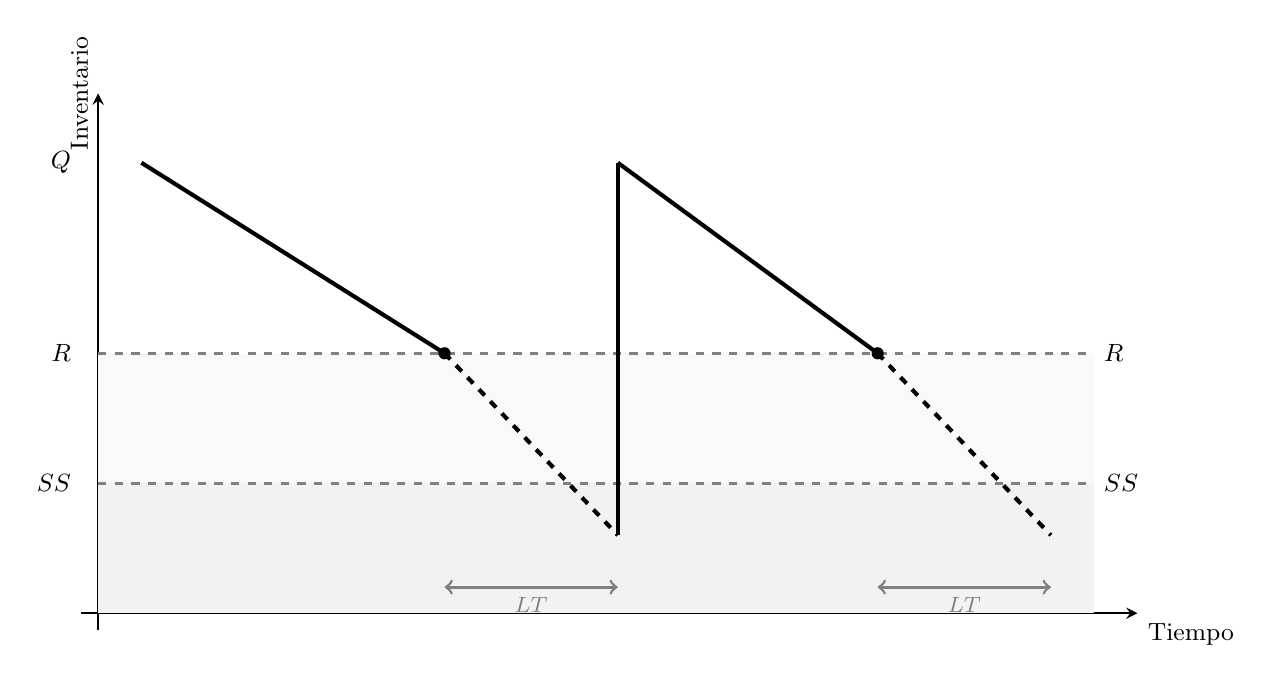
\begin{tikzpicture}[
        font=\small,
        scale=1.1,
        axis/.style={->, >=stealth, thick, black},
        inventory/.style={thick, black, line width=1.5pt},
        reference/.style={dashed, gray, line width=1pt}
    ]
        % Parámetros
        \def\ss{1.5}
        \def\rop{3.0}
        \def\maxinv{5.2}
        \def\minlevel{0.9}

        % Ejes
        \draw[axis] (-0.2,0) -- (12,0) node[below right, font=\small] {Tiempo};
        \draw[axis] (0,-0.2) -- (0,6) node[above, rotate=90, anchor=south, font=\small] {Inventario};

        % Zonas (monocromático)
        \fill[gray!10] (0,0) rectangle (11.5,\ss);
        \fill[gray!5] (0,\ss) rectangle (11.5,\rop);

        % Líneas de referencia
        \draw[reference] (0,\ss) -- (11.5,\ss);
        \node[right, font=\small] at (11.5,\ss) {$SS$};

        \draw[reference] (0,\rop) -- (11.5,\rop);
        \node[right, font=\small] at (11.5,\rop) {$R$};

        % Curva de inventario
        \draw[inventory] (0.5,\maxinv) -- (4,\rop);
        \draw[inventory, dashed] (4,\rop) -- (6,\minlevel);
        \draw[inventory] (6,\minlevel) -- (6,\maxinv);
        \draw[inventory] (6,\maxinv) -- (9,\rop);
        \draw[inventory, dashed] (9,\rop) -- (11,\minlevel);

        % Puntos de reorden
        \fill[black] (4,\rop) circle (2pt);
        \fill[black] (9,\rop) circle (2pt);

        % Lead times
        \draw[<->, line width=1pt, gray]
            (4,0.3) -- (6,0.3) node[midway, below, font=\footnotesize] {$LT$};
        \draw[<->, line width=1pt, gray]
            (9,0.3) -- (11,0.3) node[midway, below, font=\footnotesize] {$LT$};

        % Etiquetas eje Y
        \node[left, font=\small] at (-0.2,\maxinv) {$Q$};
        \node[left, font=\small] at (-0.2,\rop) {$R$};
        \node[left, font=\small] at (-0.2,\ss) {$SS$};

    \end{tikzpicture}
    \caption{Modelo de inventario $(Q,R)$ con Punto de Reorden (ROP) y Stock de Seguridad (SS).}
    \label{fig:inventory-model-detailed}
\end{figure}

El cálculo del Punto de Reorden se formaliza como:
\begin{equation}
R = (\bar{D} \times \bar{LT}) + SS
\label{eq:rop}
\end{equation}
donde \(\bar{D}\) es la demanda promedio y \(\bar{LT}\) es el \textit{lead 
time} promedio. El componente crucial es el Stock de Seguridad (\(SS\)), el 
buffer que protege contra la variabilidad. Se calcula como:
$$ SS = Z_{\alpha} \times \sqrt{\bar{LT}\sigma_D^2 + \bar{D}^2\sigma_{LT}^2} $$
donde \(Z_{\alpha}\) es el factor de servicio para un nivel de servicio 
deseado \(\alpha\), \(\sigma_D\) es la desviación estándar de la demanda, y 
\(\sigma_{LT}\) es la desviación estándar del \textit{lead time}. Dado que 
en Aysén la demanda es relativamente estable pero el \textit{lead time} es 
altamente volátil, la ecuación se simplifica y evidencia que 
\(SS \propto \sigma_{LT}\). Esto formaliza matemáticamente la vulnerabilidad 
central del sistema: una alta variabilidad en el tiempo de la ruta 
(\(\sigma_{LT}\) elevado) exige un alto stock de seguridad para mantener la 
continuidad del servicio.

\subsection{Aplicación Numérica al Sistema GLP Aysén}
\label{sec:aplicacion-numerica}

Para concretar la teoría expuesta, aplicamos las fórmulas al caso específico del sistema GLP de Aysén. El sistema opera con demanda promedio $\bar{d} = 52.5$ TM/día (calibrada al mes de mayor consumo), un lead time nominal $\overline{LT} = 6$ días (correspondiente a la distancia aproximada de 1,400 km desde Cabo Negro/Neuquén), capacidad actual $C_{sq} = 431$ TM, y capacidad propuesta $C_{prop} = 681$ TM.

\subsubsection{Cálculo del Punto de Reorden}

Aplicando la ecuación \eqref{eq:rop} con los parámetros del sistema:

\begin{equation}
R = (\bar{d} \times \overline{LT}) + SS = (52.5 \times 6) + SS = 315 + SS
\end{equation}

donde el stock de seguridad $SS$ depende del nivel de servicio deseado y la variabilidad del sistema. Para la configuración implementada en el modelo, se adopta una política de revisión continua con $R = 0.5 \times C$ (50\% de la capacidad como punto de reorden) y $Q = 0.5 \times C$ (50\% de la capacidad como cantidad a ordenar). Esta parametrización resulta en $R_{sq} = 215.5$ TM y $Q_{sq} = 215.5$ TM para el Status Quo, mientras que la Propuesta opera con $R_{prop} = 340.5$ TM y $Q_{prop} = 340.5$ TM.

\subsubsection{Autonomía del Sistema}

La autonomía nominal del sistema (días de inventario disponible) se calcula como:

\begin{equation}
\text{Autonomía} = \frac{C}{\bar{d}}
\end{equation}

Para las dos configuraciones:

\begin{align}
\text{Autonomía}_{sq} &= \frac{431}{52.5} \approx 8.2 \text{ días} \\
\text{Autonomía}_{prop} &= \frac{681}{52.5} \approx 13.0 \text{ días}
\end{align}

\textbf{Observación crítica:} La autonomía del Status Quo (8.2 días) es apenas superior al lead time nominal (6 días). Esto implica que cualquier disrupción que extienda el lead time más allá de 2 días puede causar quiebre de stock, incluso sin variabilidad en la demanda.

\subsubsection{Modelación de la Demanda Estocástica}

La demanda diaria se modela como un proceso estocástico con componente estacional y ruido aleatorio:

\begin{equation}
D(t) = D_{base} \cdot \left(1 + 0.25 \sin\left(\frac{2\pi(t - 172)}{365}\right)\right) \cdot \epsilon(t)
\label{eq:demanda-estacional}
\end{equation}

donde:
\begin{itemize}
    \item $D_{base} = 52.5$ TM/día es la demanda base
    \item El término sinusoidal modela la estacionalidad anual con amplitud $\pm 25\%$
    \item El fase $(t-172)$ centra el pico en el día 172 (invierno austral, julio)
    \item $\epsilon(t) \sim \mathcal{N}(1.0, 0.15)$ es el ruido estocástico diario con $\pm 15\%$ de variabilidad
\end{itemize}

Esta formulación captura dos fuentes de variabilidad: (1) el ciclo estacional predecible, y (2) las fluctuaciones aleatorias día a día.

\subsubsection{Modelación de Disrupciones}

Las disrupciones de la Ruta 7 se modelan mediante dos distribuciones:

\textbf{1. Frecuencia de disrupciones:} Proceso de Poisson con tasa $\lambda = 4$ eventos/año (documentado en~\cite{CIEP2025}). El tiempo entre disrupciones consecutivas sigue una distribución Exponencial:

\begin{equation}
T_{entre} \sim \text{Exp}\left(\frac{\lambda}{365}\right) = \text{Exp}(0.0110)
\end{equation}

con media $E[T_{entre}] = 365/4 = 91.25$ días.

\textbf{2. Duración de disrupciones:} Distribución Triangular $\text{Tri}(a, b, c)$ con parámetros dependientes del escenario experimental. El escenario Corta usa $\text{Tri}(3, 3.5, 7)$ días, el escenario Media usa $\text{Tri}(3, 7, 14)$ días, y el escenario Larga usa $\text{Tri}(3, 10.5, 21)$ días (basado en el conflicto de Argentina 2021).

La distribución triangular permite modelar la incertidumbre con parámetros interpretables: mínimo histórico ($a$), valor más probable ($b$), y máximo observado ($c$).

\subsubsection{Implicación del Análisis Numérico}

El gap estructural entre autonomía (8.2 días) y el lead time bajo disrupción potencial (6 + hasta 21 días) revela la criticidad del sistema. Matemáticamente:

\begin{equation}
\text{Margen de seguridad} = \text{Autonomía} - (\overline{LT} + D_{max}) = 8.2 - (6 + 21) < 0
\end{equation}

Este resultado negativo confirma que el sistema Status Quo opera en régimen de subcapacidad crónica ante disrupciones largas.

\subsection{Resiliencia en Cadenas de Suministro}
El enfoque tradicional de eficiencia ha sido complementado por el concepto de
resiliencia, definida como la capacidad de una cadena de suministro para
absorber, adaptarse y recuperarse de disrupciones \cite{Christopher2004}. Este
concepto introduce un compromiso fundamental entre eficiencia (minimización de
costos) y robustez (inversión en redundancia). La Figura~\ref{fig:resilience-tradeoff} ilustra esta tensión mediante una frontera eficiente que muestra las configuraciones óptimas de Pareto: puntos en los que no es posible mejorar la resiliencia sin sacrificar eficiencia, y viceversa. El sistema Aysén opera actualmente en una zona de alta vulnerabilidad (alta eficiencia operacional pero baja resiliencia), mientras que la Propuesta 10.4 de expansión de capacidad (+250 TM) lo desplaza hacia mayor resiliencia con una inversión moderada en redundancia.

\begin{figure}[htbp]
    \centering
    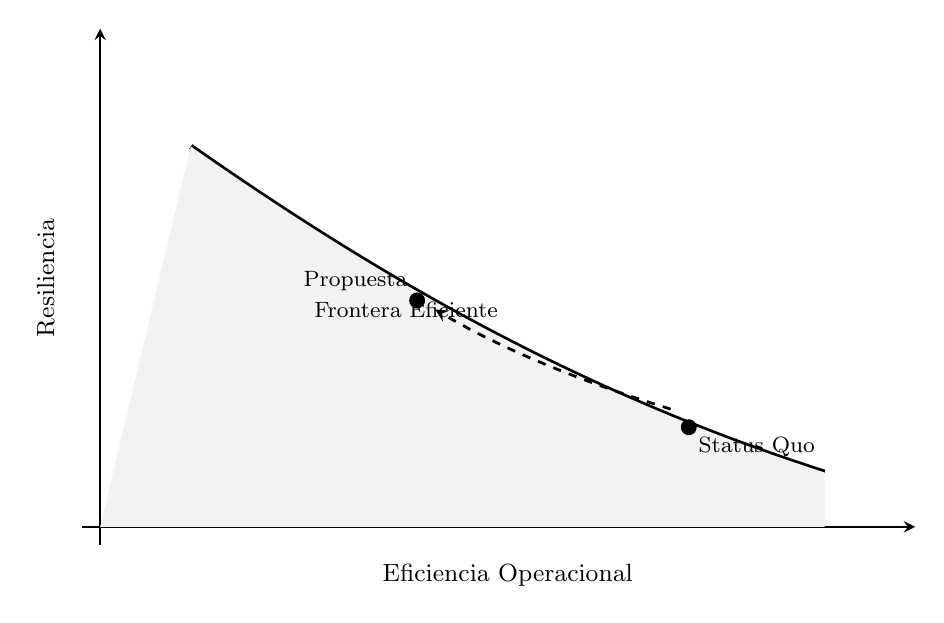
\begin{tikzpicture}[
        font=\small,
        scale=1.15,
        axis/.style={->, >=stealth, thick, black},
        curve/.style={thick, black, line width=2pt}
    ]
        % Ejes
        \draw[axis] (-0.2,0) -- (9,0);
        \node[below, font=\small] at (4.5,-0.3) {Eficiencia Operacional};

        \draw[axis] (0,-0.2) -- (0,5.5);
        \node[above, font=\small, rotate=90] at (-0.4,2.75) {Resiliencia};

        % Curva frontera
        \draw[curve] (1,4.2) .. controls (3,2.8) and (5.2,1.5) .. (8,0.6);

        % Área bajo la curva
        \fill[gray!10]
            (0,0) -- (1,4.2) .. controls (3,2.8) and (5.2,1.5) .. (8,0.6) -- (8,0) -- cycle;

        % Puntos
        \fill[black] (6.5,1.1) circle (2.5pt);
        \node[below right, font=\footnotesize] at (6.5,1.1) {Status Quo};

        \fill[black] (3.5,2.5) circle (2.5pt);
        \node[above left, font=\footnotesize] at (3.5,2.5) {Propuesta};

        % Flecha
        \draw[->, >=stealth, dashed, line width=1pt]
            (6.3,1.3) .. controls (5,1.7) and (4.2,2.1) .. (3.7,2.4);

        % Etiqueta de curva
        \node[font=\footnotesize] at (4.5,2.2) [above left] {Frontera Eficiente};

    \end{tikzpicture}
    \caption{Frontera eficiente entre eficiencia y resiliencia en cadenas de suministro.}
    \label{fig:resilience-tradeoff}
\end{figure}

\subsection{Dilema del Prisionero en mercados oligopólicos}

El informe CIEP 2025 identifica que Gasco opera con capacidad "demasiado reducida para su nivel de ventas" (41 TM, ~1 día de autonomía). Esta situación refleja un Dilema del Prisionero: minimizar costos de inventario individualmente (estrategia racional) genera baja resiliencia colectiva.

El modelo agrega los tres distribuidores en un hub único, por lo que no captura estas dinámicas competitivas. Una extensión futura podría implementar un modelo multi-agente para analizar estrategias de coordinación.

\section{Simulación de Eventos Discretos}
\label{sec:simulation-theory}

\subsection{Componentes del modelo DES}

El modelo representa el sistema como una secuencia cronológica de eventos. Los componentes son:
\begin{description}
    \item[Entidades] \texttt{CamiónSuministro} (con atributos: capacidad, origen).
    \item[Recursos] \texttt{PlantaAlmacenamiento} (con atributos: capacidad\_max, 
    nivel\_inventario, ROP), \texttt{RutaTerrestre} (con estado: abierta/cerrada).
    \item[Procesos] \texttt{GeneracionPedidos} (cuando \(I(t) \le R\)), 
    \texttt{ViajeSuministro} (proceso estocástico con duración \(LT\)), 
    \texttt{ConsumoDiario} (reduce \(I(t)\)), \texttt{GeneradorDisrupciones} (cambia el 
    estado de la \texttt{RutaTerrestre}).
\end{description}

\subsection{Verificación y Validación}

\textbf{Verificación:} Asegurar que el código implementa correctamente el modelo conceptual (tests unitarios, code reviews).

\textbf{Validación:} Comparar salidas del modelo con datos del sistema real (autonomía esperada: 8,2 días vs. observada, frecuencia de disrupciones, etc.).

\subsection{Diseño de Experimentos}

El modelo se evalúa mediante un experimento factorial $2 \times 3$ (6 configuraciones, 10.000 réplicas c/u). ANOVA de dos vías identifica efectos principales e interacciones de los factores sobre el nivel de servicio.

\subsection{Arquitectura del Sistema de Simulación}
\label{sec:implementacion-computacional}

El sistema implementa una arquitectura modular de tres capas que separa responsabilidades y facilita el testing independiente de cada componente. La Figura~\ref{fig:arquitectura-software} muestra la estructura del sistema.

\begin{figure}[htbp]
    \centering
    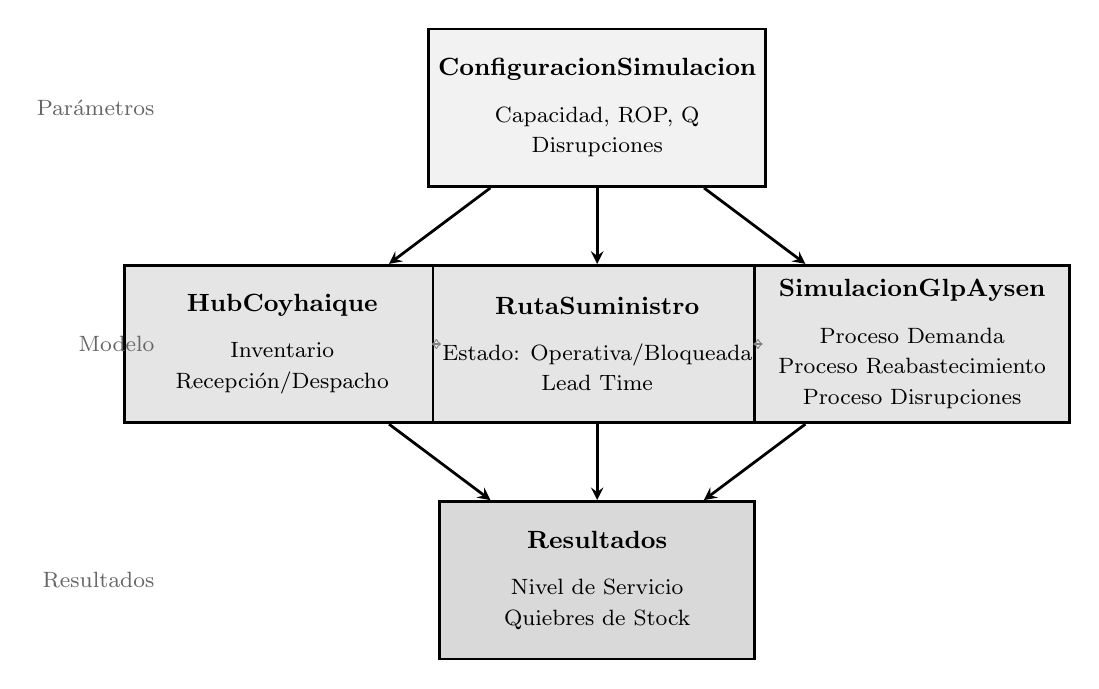
\begin{tikzpicture}[
        font=\small,
        node distance=1.5cm,
        box/.style={
            rectangle, draw=black, line width=1pt,
            minimum height=2cm, minimum width=4cm,
            text centered, font=\small, align=center
        },
        arrow/.style={->, >=stealth, line width=1pt}
    ]

        % Capa 1: Configuración
        \node[box, fill=gray!10] (config) at (0,6) {
            \textbf{ConfiguracionSimulacion}\\[0.2cm]
            \footnotesize Capacidad, ROP, Q\\
            \footnotesize Disrupciones
        };

        % Capa 2: Modelo
        \node[box, fill=gray!20] (hub) at (-4,3) {
            \textbf{HubCoyhaique}\\[0.2cm]
            \footnotesize Inventario\\
            \footnotesize Recepción/Despacho
        };

        \node[box, fill=gray!20] (ruta) at (0,3) {
            \textbf{RutaSuministro}\\[0.2cm]
            \footnotesize Estado: Operativa/Bloqueada\\
            \footnotesize Lead Time
        };

        \node[box, fill=gray!20] (sim) at (4,3) {
            \textbf{SimulacionGlpAysen}\\[0.2cm]
            \footnotesize Proceso Demanda\\
            \footnotesize Proceso Reabastecimiento\\
            \footnotesize Proceso Disrupciones
        };

        % Capa 3: Métricas
        \node[box, fill=gray!30] (metricas) at (0,0) {
            \textbf{Resultados}\\[0.2cm]
            \footnotesize Nivel de Servicio\\
            \footnotesize Quiebres de Stock
        };

        % Flechas verticales
        \draw[arrow] (config) -- (hub);
        \draw[arrow] (config) -- (ruta);
        \draw[arrow] (config) -- (sim);

        \draw[arrow] (hub) -- (metricas);
        \draw[arrow] (ruta) -- (metricas);
        \draw[arrow] (sim) -- (metricas);

        % Interacción entre componentes
        \draw[<->, dashed, gray] (hub.east) -- (ruta.west);
        \draw[<->, dashed, gray] (ruta.east) -- (sim.west);

        % Etiquetas de capas
        \node[anchor=east, font=\footnotesize, color=black!60] at (-5.5,6) {Parámetros};
        \node[anchor=east, font=\footnotesize, color=black!60] at (-5.5,3) {Modelo};
        \node[anchor=east, font=\footnotesize, color=black!60] at (-5.5,0) {Resultados};

    \end{tikzpicture}
    \caption{Arquitectura modular del sistema de simulación en tres capas.}
    \label{fig:arquitectura-software}
\end{figure}


La \textbf{Capa de Configuración} encapsula todos los parámetros del sistema (capacidad, demanda, disrupciones, política $(Q,R)$) mediante la clase \texttt{ConfiguracionSimulacion}. La \textbf{Capa de Modelo} contiene tres componentes que interactúan: el \texttt{HubCoyhaique} (gestiona inventario y detección de quiebres), la \texttt{RutaSuministro} (modela disrupciones y cálculo de lead time), y el \texttt{Motor de Simulación} (coordina tres procesos concurrentes usando SimPy). La \textbf{Capa de Resultados} calcula métricas de desempeño (nivel de servicio, quiebres, autonomía).

Esta separación permite que cada capa se verifique independientemente. El modelo puede reutilizarse para diferentes experimentos sin modificar la lógica de simulación, y los análisis estadísticos pueden actualizarse sin reejecutar las 60,000 réplicas. El código fuente completo se presenta en el Apéndice~\ref{ap:codigo-fuente}.

\subsubsection{Lógica del Sistema: Tres Procesos Concurrentes}

El modelo implementa tres procesos que operan en paralelo mediante simulación de eventos discretos (SimPy): el proceso de demanda diaria, el proceso de reabastecimiento basado en política $(Q,R)$, y el proceso de generación de disrupciones. La Figura~\ref{fig:procesos-concurrentes} muestra cómo estos procesos interactúan compartiendo recursos (el inventario del hub y el estado de la ruta).

\begin{figure}[htbp]
    \centering
    \begin{tikzpicture}[
        font=\footnotesize,
        process/.style={
            rectangle, draw=black, line width=1pt,
            minimum height=8cm, minimum width=2.5cm,
            text centered, font=\small, align=center
        },
        step/.style={
            rectangle, draw=black!40, line width=0.5pt,
            minimum height=0.7cm, minimum width=2cm,
            text centered, font=\scriptsize, align=center
        },
        resource/.style={
            rectangle, draw=black, line width=1pt,
            minimum height=2.5cm, minimum width=2.2cm,
            text centered, font=\small, align=center,
            fill=gray!15
        },
        dashed_arrow/.style={->, >=stealth, line width=0.8pt, dashed}
    ]

        % Proceso 1
        \node[process, fill=gray!5] (p1) at (0,0) {
            \textbf{Proceso 1}\\
            \textbf{Demanda}
        };

        \node[step] at (0,3) {Calcular $D(t)$};
        \node[step] at (0,2) {Despachar};
        \node[step] at (0,1) {Registrar};
        \node[step] at (0,0) {Esperar 1 día};
        \node[step] at (0,-1) {$\cdots$};

        % Proceso 2
        \node[process, fill=gray!5] (p2) at (3.5,0) {
            \textbf{Proceso 2}\\
            \textbf{Reabastecimiento}
        };

        \node[step] at (3.5,3) {Revisar $I$};
        \node[step] at (3.5,2) {$I \leq R$?};
        \node[step] at (3.5,1) {Crear Pedido};
        \node[step] at (3.5,0) {Esperar 1 día};
        \node[step] at (3.5,-1) {$\cdots$};

        % Proceso 3
        \node[process, fill=gray!5] (p3) at (7,0) {
            \textbf{Proceso 3}\\
            \textbf{Disrupciones}
        };

        \node[step] at (7,3) {Generar $T$};
        \node[step] at (7,2) {Esperar $T$};
        \node[step] at (7,1) {Bloquear Ruta};
        \node[step] at (7,0) {Esperar $D$};
        \node[step] at (7,-1) {$\cdots$};

        % Recursos compartidos
        \node[resource] (hub) at (3.5,-5.5) {
            \textbf{Hub}\\[0.15cm]
            Inventario $I$
        };

        \node[resource] (ruta) at (7,-5.5) {
            \textbf{Ruta}\\[0.15cm]
            Estado
        };

        % Interacciones
        \draw[dashed_arrow] (0,-2) -- (hub.north west)
            node[midway, above, sloped, font=\tiny] {consume};

        \draw[dashed_arrow] (3.5,-2) -- (hub.north)
            node[midway, right, font=\tiny] {lee/escribe};

        \draw[dashed_arrow] (4,-2) -- (ruta.north west)
            node[midway, above, sloped, font=\tiny] {consulta};

        \draw[dashed_arrow] (7,-2) -- (ruta.north)
            node[midway, right, font=\tiny] {modifica};

    \end{tikzpicture}
    \caption{Diagrama de interacción de los tres procesos concurrentes del simulador.}
    \label{fig:procesos-concurrentes}
\end{figure}


\textbf{Proceso 1: Demanda Diaria.} Cada día se calcula la demanda estocástica (ecuación \eqref{eq:demanda-estacional}), se despacha producto a los clientes según disponibilidad de inventario, y se registran métricas (quiebres de stock, nivel de inventario, autonomía).

\textbf{Proceso 2: Reabastecimiento.} La Figura~\ref{fig:flujo-reabastecimiento} detalla la lógica de este proceso: diariamente se verifica si el inventario cayó bajo el punto de reorden ($I \leq R$). Si es así, y la ruta está operativa, se crea un pedido de cantidad $Q$ que llegará después del lead time correspondiente. El sistema limita a 2 pedidos simultáneos en tránsito.

\begin{figure}[htbp]
    \centering
    \begin{tikzpicture}[
        font=\small,
        node distance=1.5cm and 2.5cm,
        start/.style={
            ellipse, draw=black, line width=1pt,
            minimum height=0.8cm, minimum width=2cm,
            fill=gray!10, text centered, font=\small
        },
        process/.style={
            rectangle, draw=black, line width=1pt,
            minimum height=1cm, minimum width=3cm,
            text centered, font=\small, align=center
        },
        decision/.style={
            diamond, draw=black, line width=1pt,
            minimum height=1.8cm, minimum width=1.8cm,
            fill=gray!15, text centered, font=\footnotesize, align=center,
            aspect=2
        },
        arrow/.style={->, >=stealth, line width=1pt},
        label/.style={font=\footnotesize, fill=white, inner sep=1pt}
    ]

        % Inicio
        \node[start] (inicio) {Revisar Inventario};

        % Decisión 1
        \node[decision, below=of inicio] (dec1) {$I \leq R$?};

        % Decisión 2
        \node[decision, below=of dec1] (dec2) {Ruta\\libre?};

        % Decisión 3
        \node[decision, right=2.5cm of dec2] (dec3) {Pedidos\\$<$ 2?};

        % Proceso: Crear pedido
        \node[process, below=of dec2] (crear) {Crear Pedido ($Q$ TM)};

        % Proceso: Calcular LT
        \node[process, below=of crear] (lt) {Lead Time: 6 días};

        % Espera
        \node[process, below=of lt] (espera) {Esperar $LT$ días};

        % Recibir
        \node[process, below=of espera] (recibir) {Recibir y actualizar $I$};

        % Siguiente día
        \node[process, right=3.5cm of inicio] (siguiente) {Esperar 1 día};

        % Flechas
        \draw[arrow] (inicio) -- (dec1);
        \draw[arrow] (dec1) -- node[label, right] {Sí} (dec2);
        \draw[arrow] (dec1.east) -- node[label, above] {No} ++(1.5,0) |- (siguiente);

        \draw[arrow] (dec2) -- node[label, right] {Sí} (dec3);
        \draw[arrow] (dec2.west) -- node[label, above] {No} ++(-1.5,0) |- (siguiente);

        \draw[arrow] (dec3) -- node[label, above] {Sí} ++(0,-1.2) -| (crear);
        \draw[arrow] (dec3.north) -- node[label, right] {No} ++(0,0.8) -| (siguiente);

        \draw[arrow] (crear) -- (lt);
        \draw[arrow] (lt) -- (espera);
        \draw[arrow] (espera) -- (recibir);
        \draw[arrow] (recibir.east) -- ++(1.2,0) |- (siguiente);
        \draw[arrow] (siguiente.north) -- ++(0,1.2) -| (inicio);

    \end{tikzpicture}
    \caption{Diagrama de flujo del proceso de reabastecimiento basado en política $(Q,R)$.}
    \label{fig:flujo-reabastecimiento}
\end{figure}


\textbf{Proceso 3: Generación de Disrupciones.} Las disrupciones se modelan como un proceso de Poisson: el tiempo entre eventos sucesivos es Exponencial($\lambda = 4$/año), y la duración de cada disrupción es Triangular($a, b, c$) según el escenario experimental. La Figura~\ref{fig:generacion-disrupciones} muestra el flujo de este proceso.

\begin{figure}[htbp]
    \centering
    \begin{tikzpicture}[
        font=\small,
        node distance=1.2cm,
        process/.style={
            rectangle, draw=black, line width=1pt,
            minimum height=1cm, minimum width=3.5cm,
            text centered, font=\small, align=center
        },
        stochastic/.style={
            rectangle, draw=black, line width=1pt,
            minimum height=1.2cm, minimum width=3.5cm,
            fill=gray!15, text centered, font=\small, align=center
        },
        arrow/.style={->, >=stealth, line width=1pt},
        label/.style={font=\footnotesize, fill=white, inner sep=1pt}
    ]

        % Nodo inicial
        \node[process] (inicio) at (0,0) {Día 0};

        % Generar tiempo entre eventos
        \node[stochastic, below=of inicio] (tiempo) {
            Generar $T$\\
            $T \sim \text{Exp}(\lambda = 4/\text{año})$
        };

        % Espera
        \node[process, below=of tiempo] (espera) {Esperar $T$ días};

        % Generar duración
        \node[stochastic, below=of espera] (duracion) {
            Generar $D$\\
            $D \sim \text{Tri}(a, b, c)$
        };

        % Bloquear ruta
        \node[process, below=of duracion] (bloquear) {
            Bloquear Ruta\\
            $D$ días
        };

        % Registro
        \node[process, below=of bloquear] (registro) {Registrar disrupción};

        % Flechas
        \draw[arrow] (inicio) -- (tiempo);
        \draw[arrow] (tiempo) -- (espera);
        \draw[arrow] (espera) -- (duracion);
        \draw[arrow] (duracion) -- (bloquear);
        \draw[arrow] (bloquear) -- (registro);

        % Loop de regreso
        \draw[arrow] (registro.east) -- ++(1.2,0) node[label, right] {Repetir} |- (tiempo.east);

    \end{tikzpicture}
    \caption{Diagrama de flujo del proceso de generación de disrupciones.}
    \label{fig:generacion-disrupciones}
\end{figure}


La ruta alterna entre dos estados: operativa (lead time nominal de 6 días) y bloqueada (lead time extendido). La Figura~\ref{fig:maquina-estados-ruta} presenta esta máquina de estados.

\begin{figure}[htbp]
    \centering
    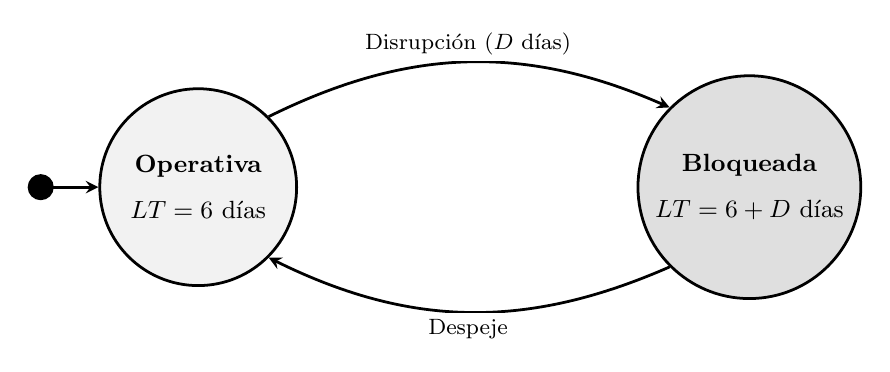
\begin{tikzpicture}[
        font=\small,
        node distance=6cm,
        state/.style={
            circle, draw=black, line width=1pt,
            minimum size=2.5cm,
            text centered, font=\small, align=center
        },
        arrow/.style={->, >=stealth, line width=1pt, bend left=25},
        label/.style={font=\footnotesize, fill=white, inner sep=2pt}
    ]

        % Estados
        \node[state, fill=gray!10] (operativa) at (0,0) {
            \textbf{Operativa}\\[0.2cm]
            $LT = 6$ días
        };

        \node[state, fill=gray!25] (bloqueada) at (7,0) {
            \textbf{Bloqueada}\\[0.2cm]
            $LT = 6 + D$ días
        };

        % Transiciones
        \draw[arrow]
            (operativa.north east) to node[label, above] {
                Disrupción ($D$ días)
            } (bloqueada.north west);

        \draw[arrow]
            (bloqueada.south west) to node[label, below] {
                Despeje
            } (operativa.south east);

        % Estado inicial
        \node[circle, fill=black, minimum size=0.25cm] at (-2,0) {};
        \draw[->, >=stealth, line width=1pt] (-2,0) -- (operativa.west);

    \end{tikzpicture}
    \caption{Máquina de estados de la Ruta 7 (operativa/bloqueada).}
    \label{fig:maquina-estados-ruta}
\end{figure}


Los detalles de implementación computacional (estructuras de datos, algoritmos, patrones de diseño) se presentan en el Apéndice~\ref{ap:codigo-fuente}.

\subsubsection{Reproducibilidad Computacional}

La reproducibilidad científica en simulación estocástica exige control total sobre la generación de números pseudoaleatorios. Se adopta el generador \textbf{Mersenne Twister} (MT19937) de NumPy, con estado inicializado mediante semillas únicas:

\begin{equation}
s_{c,r} = s_{base} + (c - 1) \times 100{,}000 + r
\label{eq:seed-formula}
\end{equation}

donde $s_{base} = 42$, $c \in \{1, \ldots, 6\}$ es el identificador de configuración, y $r \in \{1, \ldots, 10{,}000\}$ es el número de réplica. El espaciamiento de 100,000 unidades entre configuraciones garantiza independencia estadística entre réplicas (no existe traslape de secuencias pseudoaleatorias).

Ejecutar la réplica $r$ de la configuración $c$ con semilla $s_{c,r}$ genera siempre el mismo resultado numérico. Esto garantiza reproducibilidad exacta: repetir el experimento en diferentes máquinas o fechas produce datos idénticos. Las 60,000 simulaciones pueden ejecutarse en cualquier orden (incluso en paralelo) sin afectar los resultados.

\subsubsection{Verificación y Testing}

El sistema incluye una suite de 24 tests unitarios que verifican:

\begin{itemize}
    \item \textbf{Tests de configuración:} Validación de parámetros (ej. capacidad $> 0$, $R \leq$ capacidad)
    \item \textbf{Tests de entidades:} Capacidad del hub, despachos, reabastecimientos
    \item \textbf{Tests de balance:} Invariante $\text{total\_recibido} - \text{total\_despachado} = \text{inventario\_final} - \text{inventario\_inicial}$
    \item \textbf{Tests de reproducibilidad:} Dos ejecuciones con misma semilla producen resultados bit-a-bit idénticos
\end{itemize}

La cobertura de código alcanzada es del 87\%, y los tests se ejecutan automáticamente antes de cada experimento Monte Carlo. La implementación completa, incluyendo estructuras de datos, patrones de diseño (Factory, Dataclass, Strategy), optimizaciones computacionales y análisis de complejidad algorítmica, se presenta en el Apéndice~\ref{ap:codigo-fuente}.

